% !TEX TS-program = pdflatex
% !TEX encoding = UTF-8 Unicode

% This is a simple template for a LaTeX document using the "article" class.
% See "book", "report", "letter" for other types of document.

\documentclass[8pt]{article} % use larger type; default would be 10pt

\usepackage[utf8]{inputenc} % set input encoding (not needed with XeLaTeX)
\usepackage{bchart}
\usepackage{longtable}
\usepackage{pgfgantt}
\usepackage{calendar} % Use the calendar.sty style
\usepackage{calc}
\usepackage{ifthen}
\usepackage{tkz-base}
\usepackage{pdfpages}
\usepackage{hyperref}
\usepackage{pgfplots}
\usepackage{tkz-kiviat,numprint,fullpage} 
\usepackage{pgfplotstable} 
\usetikzlibrary{arrows}
\usepackage{paralist} % very flexible & customisable lists (eg. enumerate/itemize, etc.)
\usepackage{dcolumn}
\usepackage{booktabs}
\usepackage{lscape}
\usepackage{pgf-pie}
\usepackage{verbatim}
\usepackage{animate}
\usepackage{sfmath}

%%% Examples of Article customizations
% These packages are optional, depending whether you want the features they provide.
% See the LaTeX Companion or other references for full information.

\usepackage{textcomp}
%\usepackage{hyperref}

%%% PAGE DIMENSIONS
\usepackage{geometry} % to change the page dimensions
\geometry{a4paper} % or letterpaper (US) or a5paper or....
% \geometry{margin=2in} % for example, change the margins to 2 inches all round
% \geometry{landscape} % set up the page for landscape
%   read geometry.pdf for detailed page layout information

\usepackage{graphicx} % support the \includegraphics command and options

% \usepackage[parfill]{parskip} % Activate to begin paragraphs with an empty line rather than an indent

%%% PACKAGES
\usepackage{booktabs} % for much better looking tables
\usepackage{array} % for better arrays (eg matrices) in maths
\usepackage{paralist} % very flexible & customisable lists (eg. enumerate/itemize, etc.)
\usepackage{verbatim} % adds environment for commenting out blocks of text & for better verbatim
\usepackage{subfig} % make it possible to include more than one captioned figure/table in a single float
% These packages are all incorporated in the memoir class to one degree or another...

%%% HEADERS & FOOTERS
\usepackage{fancyhdr} % This should be set AFTER setting up the page geometry
\pagestyle{fancy} % options: empty , plain , fancy
\renewcommand{\headrulewidth}{0pt} % customise the layout...
\lhead{}\chead{}\rhead{}
\lfoot{}\cfoot{\thepage}\rfoot{}

%%% SECTION TITLE APPEARANCE
\usepackage{sectsty}
\allsectionsfont{\sffamily\mdseries\upshape} % (See the fntguide.pdf for font help)
% (This matches ConTeXt defaults)

%%% ToC (table of contents) APPEARANCE
\usepackage[nottoc,notlof,notlot]{tocbibind} % Put the bibliography in the ToC
\usepackage[titles,subfigure]{tocloft} % Alter the style of the Table of Contents
\renewcommand{\cftsecfont}{\rmfamily\mdseries\upshape}
\renewcommand{\cftsecpagefont}{\rmfamily\mdseries\upshape} % No bold!

%%% END Article customizations

%%% The "real" document content comes below...

%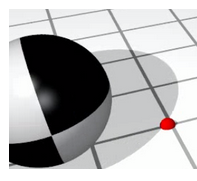
\includegraphics[width=.2\textwidth]{Logo.png}

\title{Finance}
\author{\copyright Frederic Kerdraon}
%\date{} % Activate to display a given date or no date (if empty),
         % otherwise the current date is printed 

%\addtobeamertemplate{frametitle}{}{%
%\begin{tikzpicture}[remember picture,overlay]
%\node[anchor=north west,yshift=2pt] at (current page.north west) {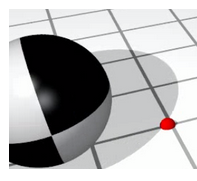
\includegraphics[height=0.8cm]{Logo1}};
%\end{tikzpicture}}

\begin{document}
\maketitle
\tableofcontents

%%%%%%%%%%%%%%%%%%%%%%%%%%%%%%%%%%%%%%%%%%%%%%%%%%%%%%%%%%%%%%%%%%%%%%%%%%%%%%%%%%%%%%%%%%%%%%%%%%%%%%%%%%%%%%%%%%%%%%%%%%%%%%%%%%%%%%%%%%%%%%%%%%%%%
\section{Asset Liability Management}

\subsection{Kapital}

\subsubsection{Table}
History of the Kapital is available in the database (select * from kapital)

%$\lim_{x \to \infty} \exp(-x) = 0$
%$\lim_{x \to \infty} \exp(-x) = 0$
%K: Kapital\\
%A: Assets\\
%L: Liabilities\\
%K = A-L\\
%L = K/L\\

\subsubsection{Graph}
A graph of the kapital and not income and charges cumulated should be easy to build.
Say a readKapital which would select the cash balance + all the other stuff like assets - liabilities
Better do it with Latex than with the C++ 

\subsubsection{History}
{\footnotesize
Historical graph of the kapital, liab and assets, yearly ALM management\\
%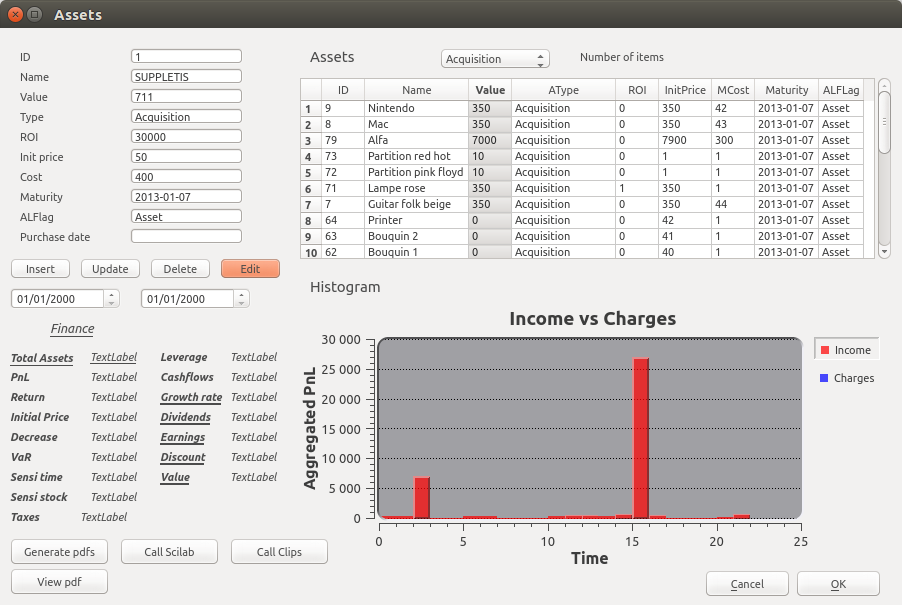
\includegraphics[width=.8\textwidth]{Assets.png}
}

\subsubsection{Definitions}
{\footnotesize
Vp: value weight (basically the value of the asset against the total value - to be replaced by InitPrice)\\
Rp: return weight (the return compared to the total returns)\\
Cp: cost weight (the maintenance cost compared to the total maintenance\\
Vd: historical deprecation of value (the Value compared to the InitPrice\\
R/V: monthly rentability (the return minus the maintenance)\\}

\subsubsection{Ratios}
{\footnotesize
Vp = value/Totalvalue\\
Rp = return/Totalreturn\\
Cp = cost/Totalmaintenance\\
Vd = value/Initprice\\
R/V = return/Value\\}

\subsubsection{Formulas}

{\footnotesize
$\lim_{x \to \infty} \exp(-x) = 0$\\
}

\subsection{Assets}

\subsubsection{Data}
The top 5 assets are listed sorted by value, but the totals are given for all the assets as of today\\
%I KNOW THERE ARE SOME FUNNY NUMBERS!!!\\

\begin{longtable}{|c|c|c|c|c|c|c|c|c|c|c|c|}
\hline
\multicolumn{12}{|c|}{Assets} \\
\hline
Type & Name & Maturity & Value & Return & Cost & InitPrice & vp & rp & mp & dv & PnL(R/V)\\
\hline
Boat & Acquisition & 2013-01-07 & 8.33333333333333 & 50 & 400 & 30000 & 63 & 0 & 3 & 83 & 0\\
\hline
CEL & Acquisition & 2013-01-07 & 0.161 & 50 & 400 & 30000 & 1 & 0 & 3 & 1 & 0\\
\hline
LDD & Acquisition & 2013-01-07 & 0.014 & 50 & 400 & 30000 & 0 & 0 & 3 & 0 & 0\\
\hline
TITR & Acquisition & 2013-01-07 & 0.0156666666666667 & 50 & 400 & 30000 & 0 & 0 & 3 & 0 & 0\\
\hline
PRED & Acquisition & 2013-01-07 & 0.0466666666666667 & 50 & 400 & 30000 & 0 & 0 & 3 & 0 & 0\\
\hline
 ... & ... & ... & ... & ... & ... & ... & ... & ... & ... & ... & ...\\
\hline
& Total assets & 273076 & 39593 & 7991 & 10273 & & & & & & -2282\\
\hline
\end{longtable}


\subsubsection{Graph}
\begin{bchart}[min=0,max=25,step=5,unit=k\texteuro]
\bcbar[label=Boat]{0.00833333333333333}\\
\smallskip
\bcbar[label=CEL]{0.000161}\\
\smallskip
\bcbar[label=LDD]{1.4e-05}\\
\smallskip
\bcbar[label=TITR]{1.56666666666667e-05}\\
\smallskip
\bcbar[label=PRED]{4.66666666666667e-05}\\
\smallskip
\end{bchart}
;

\subsubsection{Cheese}
\begin{tikzpicture}[scale=2]
\foreach \p/\t in {
72 / Boat-17k\texteuro -0\ ,
2 / CEL-0.483k\texteuro -0\ ,
0 / LDD-0.042k\texteuro -0\ ,
0 / TITR-0.047k\texteuro -0\ ,
0 / PRED-0.14k\texteuro -0\i ,
}
  {
\setcounter{a}{\value{b}}
\addtocounter{b}{\p}
\slice{\thea/100*360}
          {\theb/100*360}
          {\p\%}{\t}
  }
\end{tikzpicture}


\subsubsection{Kiviat}
\begin{tikzpicture}
\tkzKiviatDiagramFromFile[
        scale=.5,
        label distance=.5cm,
        gap     = 1,
        label space=3,  
        lattice = 10]{assets.dat}
\tkzKiviatLineFromFile[thick,
                       color      = blue,
                       mark       = ball,
                       ball color = blue,
                       mark size  = 4pt,
                       fill       = blue!20]{assets.dat}{2}
\tkzKiviatLineFromFile[thick,
                       color      = red,
                       mark       = ball,
                       ball color = red,
                       mark size  = 4pt,
                       fill       = red!20]{assets.dat}{1}     
\end{tikzpicture}

Seems like the assets Cheese 

\subsection{Liabilities}
The top 4 liabilities are listed but the totals are given for all the liabilities\\

\subsubsection{Table}
\begin{longtable}{|c|c|c|c|c|c|c|c|c|c|c|c|}
\hline
\multicolumn{12}{|c|}{Liabilities} \\
\hline
Type & Name & InitPrice & Value & Return & Cost & Maturity & vp & rp & mp & dv & PnL\\
\hline
Boat-mortgage & mortgage & 30000 & 13440 & 0 & 1 & 2013-01-07 & 55 & 0 & 25 & 44 & 0\\
\hline
Car-mortgage & mortgage & 7000 & 2287 & 0 & 1 & 2013-01-07 & 9 & 0 & 25 & 32 & 0\\
\hline
Dad-mortgage & mortgage & 5000 & 5000 & 0 & 1 & 2013-01-07 & 20 & 0 & 25 & 100 & 0\\
\hline
Mum-mortgage & mortgage & 3500 & 3500 & 0 & 1 & 2013-01-07 & 14 & 0 & 25 & 100 & 0\\
\hline
 ... & ... & ... & ... & ... & ... & ... & ... & ... & ... & ... & ...\\
\hline
& Total & 45500 & 24227 & 0 & 4 & & & & & & -4\\
\hline
\end{longtable}

\subsubsection{Graph}
\begin{bchart}[min=0,max=13,step=2,unit=k\texteuro]
\bcbar[label=Boat-mortgage]{13.44}\\
\smallskip
\bcbar[label=Car-mortgage]{2.287}\\
\smallskip
\bcbar[label=Dad-mortgage]{5}\\
\smallskip
\bcbar[label=Mum-mortgage]{3.5}\\
\smallskip
\end{bchart}

\subsubsection{Chart}
%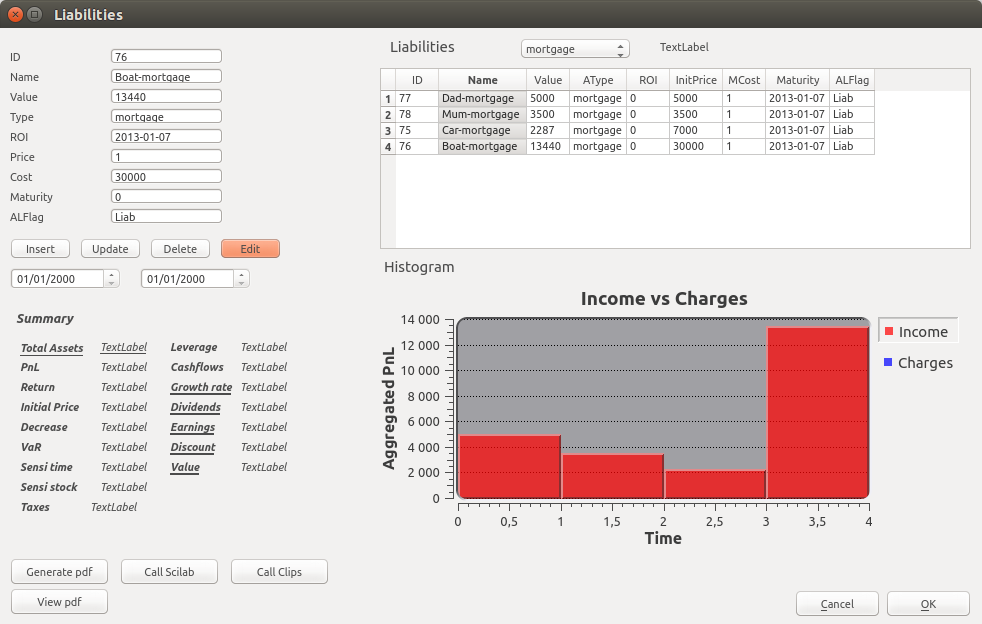
\includegraphics[width=.8\textwidth]{Liabilities.png}
\subsubsection{Cheese}
\begin{tikzpicture}[scale=2]
\foreach \p/\t in {
55 / Boat-mortgage- 13 k\texteuro ,
9 / Car-mortgage- 2 k\texteuro ,
20 / Dad-mortgage- 5 k\texteuro ,
14 / Mum-mortgage- 3 k\texteuro ,
}
  {
\setcounter{a}{\value{b}}
\addtocounter{b}{\p}
\slice{\thea/100*360}
          {\theb/100*360}
          {\p\%}{\t}
  }
\end{tikzpicture}


\section{Cashflows}

%\subsection{Management summary}

All cashflows from history are being used here\\

\subsubsection{Table}
\begin{longtable}{|c|c|c|c|c|}
\hline
\multicolumn{5}{|c|}{Cashflows} \\
\hline
Category & Debit & Credit & PnL \\
\hline
 ... & ... & ... & ...\\
\hline
 Total &  &  & 0 \\
\hline
\end{longtable}

\subsubsection{Graph}
%\begin{bchart}[min=0,max=0,step=0,unit=k\texteuro]
\end{bchart}


\end{document}

